\section{system overview and architecture}

The project is a five-degree-of-freedom (5-DOF) robotic arm that integrates a mechanical robotic arm structure, servo motors, an ESP32 microcontroller, a gripper mechanism and an object detection system using sensors. These components work together and the main process  is to identify the target object, determine its position, move the robotic arm to the required location, pick the object and place it inside a designated container. The overall system combines mechanical design, embedded control and inverse kinematics concepts to achieve the required pick-and-place operation. 

\subsection{System Overview}

This robotic arm is a 5 DOF system which consists of five joints and two links and end effector.  Servo motors are used to control each joint movement and the end effector (gripper) reaches the required position to pick and place the objects within the defined workspace. The gripper mechanism is used to grasp and release the object from one place to another.

The main control unit of this robotic arm is the ESP32 microcontroller. The main purpose of it is to gather the required movement information  of the five joints and generate the control signals for the servo motors and control the all joints of the robotic arm and the gripper mechanism.  
 
The object detection in this robotic design is mainly done by the IR sensor. It identifies the arrival of the object to the defined position and  according to that it determines the information required for the pick-and-place operation. The information which gets by the IR sensor will be provided to the control system. After getting this information about the object, the required joint angles using inverse kinematics based on the position of the end effector. 

\subsection{System Architecture}

The overall system architecture of this robotic arm includes a few main units such as ESP32 microcontroller, servo motors and control system, IR sensor and the object detection system and the arm structure. All these units are interconnected together and work as a complete system that can perform required pick-and-place operation. 


\begin{figure}[htbp]
    \centering

    \begin{tikzpicture}[
        node distance=8mm,
        box/.style={
            rectangle,
            draw,
            rounded corners,
            minimum width=42mm,
            minimum height=9mm,
            align=center
        },
        arrow/.style={
            -{Stealth},
            thick
        }
    ]

    \node[box] (sensor) {Object Detection\\Using IR Sensor};

    \node[box, below=of sensor] (position) {Position Information};

    \node[box, below=of position] (esp32) {ESP32 Micro-controller};

    \node[box, below=of esp32] (ik) {Inverse Kinematics};

    \node[box, below=of ik] (servo) {Servo Motor Control};

    \node[box, below=of servo] (arm) {5-DOF Robotic Arm};

    \node[box, below=of arm] (operation) {Grasp and\\Pick-and-Place};

    \draw[arrow] (sensor) -- (position);
    \draw[arrow] (position) -- (esp32);
    \draw[arrow] (esp32) -- (ik);
    \draw[arrow] (ik) -- (servo);
    \draw[arrow] (servo) -- (arm);
    \draw[arrow] (arm) -- (operation);

    \end{tikzpicture}

    \caption{Overall system flow of the proposed pick-and-place robotic arm}
    \label{fig:system_flow}

\end{figure}

\begin{figure}[htbp]
    \centering
    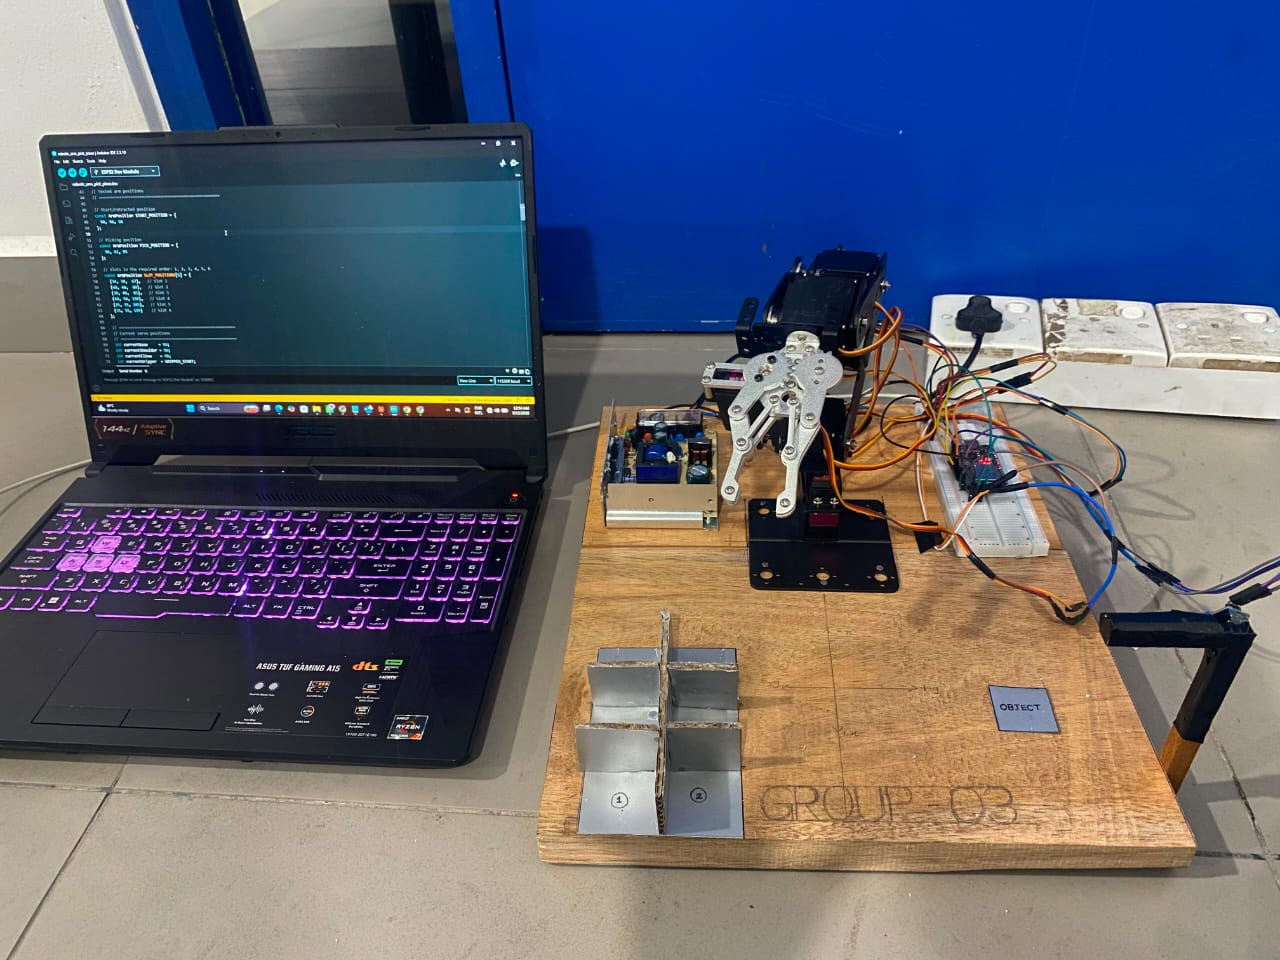
\includegraphics[width=\columnwidth]{figures/system architecture.jpeg}
    \caption{Overall system architecture of the 5-DOF pick-and-place robotic arm}
    \label{fig:system architecture}
\end{figure}


\subsection{Working Principle}

The working process of the proposed system consists of several stages. As the first step the ESP32 and the connected servo motors are initialized. The initial position of the robotic arm is predefined and the required system parameters such as angles of each joint are loaded before starting the operation.

The object detection is done by using an IR sensor at the predefined detection position. The main process is identifying the object by emitting infrared radiation and detecting the reflected signal from the object. When an object is detected by the sensor within the sensing range, it provides a corresponding signal to the ESP32 and this signal initiates the required pick-and-place operation. 

Inverse kinematics is used to calculate the joint angles based on the desired position of the robotic arm. After object detection, the control algorithm determines the joint configurations and ESP32 sends the control signals to the servo motors to move correctly toward the calculated pick position. 

When the end effector reaches the required object picking position which is calculated before, the gripper is activated and grasps the target object. After the object grasp, the gripper remains closed until the object is in the correct position. The gripper will securely hold the object while the robotic arm moves toward the target position and then releases the object.

After successfully picking the object the arm will move to the predefined target location which is determined using inverse kinematics calculations. The servo motors are controlled according to the joint angles and required joint configuration to place the object in the correct place by positioning the end effector correctly. 

The gripper opens to release the object when the end effector reaches the target location correctly. After releasing the object in the correct position, the robotic arm returns into the predefined initial position for the next pick-and-place process. 
